
\begin{question}
In a game, there is a 13\% chance to win a round. You will play 206
rounds.
\begin{answerlist}
  \item What is the probability of winning exactly 24 rounds?
  \item What is the probability of winning at least 18 but at most 35 rounds?
\end{answerlist}
\end{question}

\begin{solution}
We use the formula for binomial probabilities.
\[P(X=k) = {n \choose k} (p)^{k}(1-p)^{n-k} \]
\[P(X=24) = {206 \choose 24} (0.13)^{24}(1-0.13)^{206-24} \]
\[P(X=24) = {206 \choose 24} (0.13)^{24}(0.87)^{182} \]
\[P(X=24) = 0.0728\]

Find the mean. \[\mu = np = (206)(0.13) = 26.78 \] Find the standard
deviation.
\[\sigma = \sqrt{np(1-p)} = \sqrt{(206)(0.13)(1-0.13)} = 4.8269 \] Make
a sketch, specifically try to picture whether you need to add or
subtract 0.5 for the continuity correction.

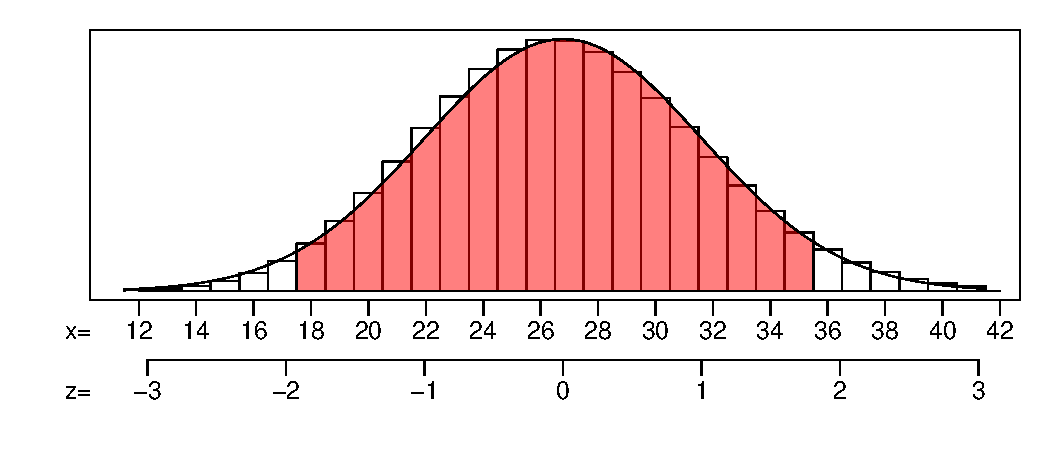
\includegraphics{binom_norm_sketch-1.pdf} Find the \(z\) scores.
\[z_1 = \frac{17.5-26.78}{4.8269} = -1.92 \]

\[z_2 = \frac{35.5-26.78}{4.8269} = 1.81 \] Calculate the probability.
\[P(18\le X \le 35) = \Phi(1.81) - \Phi(-1.92) = 0.9375 \]
\begin{answerlist}
  \item \(P(X=24) = 0.0728\)
  \item \(P(18 \le X \le 35) = 0.9375\)
\end{answerlist}
\end{solution}

